
\begin{figure*}[t]
    \centering
    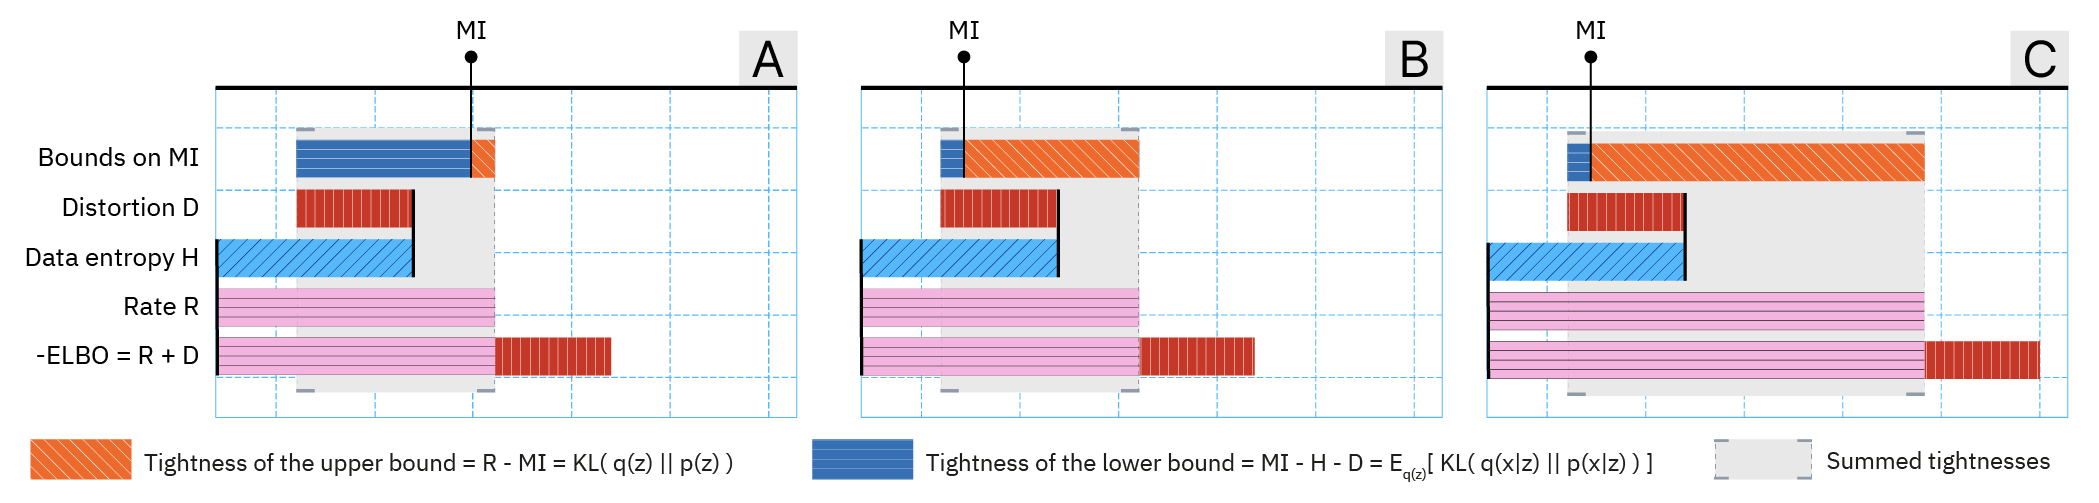
\includegraphics[width=\textwidth]{images/marginal-kl-diagram.png}
    \caption{The diagrams illustrate three scenarios with different trade-offs in information theoretic quantities. Moving between scenario A and B keeps the ELBO, rate \textit{and} distortion fixed, while the level of MI varies within the range defined by its variational bounds (denoted with the grey area). This variability allows for one scenario (B) to have a higher level of marginal KL relative to the other scenario (A). This illustrates that marginal KL is an axis of variation not accounted for in the information theoretic RD-view on VAEs. Moving from scenario B to C does \textit{not} keep the RD-view (and thus ELBO) fixed and shows the potential hazardous situation where rate is elevated merely at the cost of marginal KL, without effectively diminishing distortion nor increasing MI. This scenario may seem predictably worse (after all, ELBO is worse), but it shows a caveat of techniques that focus on targeting higher rate solutions as a proxy to higher MI.}
    \label{fig:marginal-kl-diagram}
\end{figure*}

\section{Intrinsic Criticism of VAEs}\label{sec:intrinsic}


% On LL
The most common intrinsic evaluation metric for density estimation is the log-likelihood (LL) of the model given a heldout sample of the data. The LL of a VAE is intractable, hence it is common to resort to Monte Carlo (MC) estimates through importance sampling \citep[IS;][]{robert2004monte}. 
%An often encountered transformation of log-likelihood in the realm of NLP is the perplexity per token, which exaggerates differences in log-likelihood. 
While importance weighted LL \citep[IW LL;][]{burda2015importance} gives insight into the extent to which the marginal $p_X$ matches the implicit distribution $q_X$ on average  (criterion \enumone), it falls short in providing intuition for trade-offs made in the model regarding the usage of $Z$ that we practically care about (criteria \enumtwo \& \enumthree).

% On LL not measuring anything related to Z
One example of a failure mode regarding criterion \enumtwo that need not be detected by IW LL is that of a model $p_{XZ}$ in which the latent variable $Z$ and observed variable $X$ are independent. This has been reported to occur in cases where the observational model is flexible enough to model $X$ without making use of $Z$, which establishes the consequence of a true posterior $p_{Z|X=x}$ that is independent of the data and is said to have \textit{collapsed to the prior} \citep{chen2016variational, bowman2015generating}. Due to this independence, VI finds a trivial optimum where $q_{Z|X=x}$ reduces to $p_Z$, perfectly recovering  the collapsed $p_{Z|X=x}$ for every $x \in \Omega_X$.  % the optimisation criterion of VI $\KL(q_{Z|X=x}||p_{Z|X=x})$ can be optimised by mimicking this behaviour with the inference model: $q_{Z|X=x}$ reduces to $p_Z$, for every $x \in \Omega_X$. %In this scenario, the generative model becomes an exact likelihood model.
% On RD & bounds on MI
Motivated by this observation, \citet{alemi2018fixing} develop a view over the two axes the expected ELBO naturally decomposes into: the rate-distortion (RD) plane.\footnote{The expected ELBO can be rewritten as $-D - R$, where $\mathbb E_{x \sim q_X}[\KL(q_{Z|X=x}||p_Z)]$ is the rate $R$ and the distortion $D$ is $\mathbb E_{x \sim q_{X}, z \sim q_{Z|X=x}}[\log p_{X|Z=z}(x)]$.} They demonstrate that these two quantities parametrically determine the unique variational bounds between which the mutual information (MI) between the observed variable $X$ and latent variable $Z$ under $q_{ZX}$ is guaranteed to exist for a given parametric family. This leads to the insight that for any given ELBO level, the RD ratio may vary and so may the level of MI (quantitatively associated with criterion \enumtwo). 
%This decomposition has led to a more frequent reporting of RD values for intrinsic evaluation of VAEs.

% The missing axis in RD: marginal KL
While the RD decomposition and its relation to the bounds on MI leads to an expanded intrinsic evaluation with regards to the goals outlined in \rsec{background}, a closer look at these bounds reveals that there is a degree of freedom the decomposition through the lens of $q_{ZX}$ does not account for, and which is directly relevant to criterion \enumthree: $q_Z$ matching $p_Z$. This can be quantified as the KL from the prior $p_Z$ to the marginal $q_Z$ \citep[a.k.a. \textit{marginal KL};][]{hoffman2016elbo} and can be interpreted as the tightness of the upperbound on MI, the rate, to the true MI. And, importantly, it may vary relative to the tightness of the lowerbound at fixed ELBO \textit{and} fixed rate-distortion ratio (see Figure \ref{fig:marginal-kl-diagram}A \& B).
% On bent RD curves
Furthermore, let us move from the theoretical situation where we reason in terms of fixed ELBO levels to a more realistic scenario where the optimal ELBO level at different RD ratios for a given parametric family is more likely to be defined by a bent RD-curve. In this scenario, the marginal KL may vary \textit{independently} of the tightness of the lowerbound on MI. This is practically relevant as there are numerous optimisation techniques that directly or indirectly aim at solutions that lay on segments of or form points on the RD contour defined for a parametric family \citep[e.g. ][]{kingma2016improved, pelsmaeker2019effective, chen2016variational, alemi2018fixing}. This thus potentially comes at the cost of compromised consistency and translates to higher marginal KL (Figure \ref{fig:marginal-kl-diagram}C).
%\cbnote{Perhaps one will question: why do we need marginal KL in this scenario if we can already see that the ELBO is worse. Well, the focus of this argument is not so much to push for marginal KL as a metric itself, but rather to note that we should be suspicious of artificially pushed high rate solution, which apparently is not that obvious given that papers report these higher rate higher ELBO solutions (e.g. Optimus paper).} %\wanote{To make sure I didn't miss something subtle in the argument: B and C \emph{both} illustrate that an increase in marginal KL reduces MI (right?); in addition, C illustrates (a common setting/strategy),  where one sacrifices ELBO in favour of rate hoping for higher MI, but  possibly not realising that all they may be getting is the marginal KL part of the rate.  If am on track, I'd say these arguments can be made quite explicitly in text and in the caption of the Figure. (I am biased towards big self-contained captions :D).}\\
%\cbnote{Note works of Zhao in the optimisation domain}
% In other words, since R only \textit{upper bounds} MI, targeting or reporting an increased R solution cannot disclose the potential existence of an accompanied compromised marginal approximation $q_Z$. 
%
% On problems beyond theoretical framework of R, D & K
%Besides the above said theoretical hiatus in the information theoretic intrinsic evaluation view, 
Considering a more complete view of RD together with marginal KL or MI can still lead to difficulties: it is hard to obtain good estimates of those quantities  due to their dependence on the marginal $q_Z$, which is expensive to estimate and empirically bounded by $\log N$ \citep{Song2020Understanding}. % causing the range in which estimates can be made to be small. 
On the other hand, even if we had perfect estimates at our disposal, reasoning on trade-offs between these quantities or proxies such as MMD is hard. And lastly--and possibly most importantly--none of these intrinsic metrics are explicitly designed to capture characteristics a practitioner may practically care about.

%\wanote{For MNIST, we can easily visualise problems such as 'large marginal KL'. We can generate samples group them in a grid. For a bad model, the aggregated digits won't look like digits. It might give the reader a sense of why we care? Perhaps it would belong to a subsection of Section 5, but if we will have it, we can mention it here already.}